\subsubsection{Pixels and Filters}
\begin{itemize}[--]
	\item An image contains a discrete number of pixels
	\item An image is a function $\mathbb{R}^2\to\mathbb{R}^M$
	\item $f(x,y)$ gives the intensity at position $(x,y)$


	\item \textbf{Filtering}: forming a new image whose pixels are a combination of the original image's pixel values
	\item We filter to modify or enhance image properties (super-resolution, in-painting, de-noising)
	\item \textbf{2D Discrete-Space Systems (Filters)}
		$$f(n,m)\to \text{System }\mathcal{S} \to g(n,m)$$ 
		$$g=\mathcal{S}(f),\text{ } g(n,m)=\mathcal{S}\{f(n,m)\}$$
		$$f(n,m)\xrightarrow{\mathcal{S}} g(n,m)$$
	\item \textbf{Moving average}: create a series of averages of different subsets of the full data set
	\item An example of a filter is the moving average where you take the average over a $3\times 3$ subset of pixels
		$$g(n,m)=\frac{1}{9}\sum_{k=n-1}^{n+1}\sum_{l=m-1}^{m+1} f(k,l)$$
	\begin{center}
		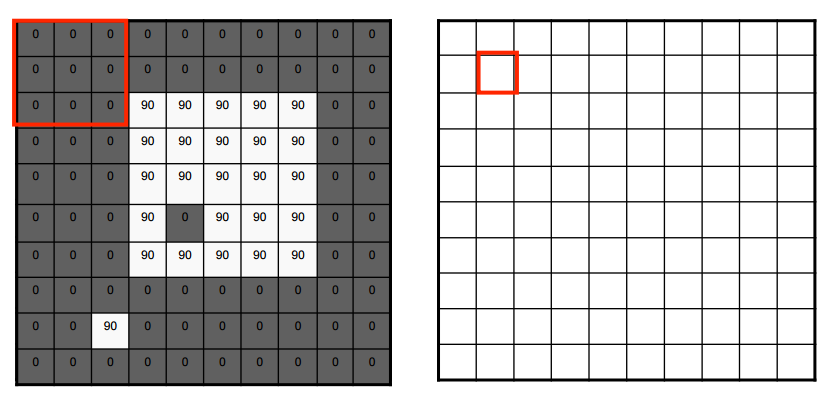
\includegraphics[scale=0.5]{sections/cs131/1-cameras/movingaverage_3x3.png}
	\end{center}

	\item Another simple filter is segmenting an image based on a threshold of pixel intensity
	$$g(n,m)=\begin{cases}
		255, &f(n,m)>100\\
		0, &\text{otherise}
	\end{cases}$$
	\item This threshold will seperate pixels whose intensities are greater than $100$ into two categories: black (255), or white (0).

	\item There are many ways to classify systems:
	\begin{itemize}[--]
		\item Amplitude properties
		\begin{itemize}[--]
			\item Linearity
			\item Stability
			\item Invertibility
		\end{itemize}

		\item Spatial properties
		\begin{itemize}[--]
			\item Causality
			\item Separability
			\item Memory
			\item Shift invariance
			\item Rotation invariance
		\end{itemize}
	\end{itemize}

	\item \textbf{Shift invariance}: if any input into a system $x(t)$ produces the output $y(t)$ then upon introduction of a shift to the input, let the shift be $\delta$, $x(t+\delta)$ results in a shifted output $y(t+\delta)$. 
	\item If $f(n,m)\xrightarrow{\mathcal{S}} g(n,m)$ then $f(n-n_0, m-m_0)\xrightarrow{\mathcal{S}} g(n-n_0, m-m_0)$ for every input image $f(n,m)$ and shifts $n_0, m_0$.
	\item \textbf{Linear filtering}: A system $\mathcal{S}$ is a linear system iff it satisfies the superposition property (additivity and homogeneity):
		$$\mathcal{S}(\alpha f_1 + \beta f_2) = \alpha\mathcal{S}(f_1) + \beta\mathcal{S} (f_2)$$
	\item Moving average isn't a linear system (TODO: need justification)
	\item Thresholding isn't a linear system, fails additivity. $f_1 < T, f_2 < T$ while $f_1+f2 > T$
	\item TODO: Impulse Resposne
	\item 
\end{itemize}